\section{Multitouch Table}
You will be assimilated (see figure \ref{fig:mtdiagram}). 
This
particular
Rear
Diffused
Illumination
Multi‐touch
design
used
a
cabinet
made
of
core‐ten
steel
that
had
recessed
cabinet
cooling
fans
and
access
panel
on
the
rear
vertical
wall.

The
touch
surface
was
made
of
1⁄2
inch
polycarbonate
with
an
adhesive
projection
film
applied
to
the
underside
of
the
touch
surface
that
acted
as
a
diffuser
for
the
projector.

A
TUIO
Client
Application
is
projected
from
the
underside
of
the
touch
surface
onto
this
diffuser.

This
is
the
image
that
the
user
will
interact
with.
Depending
on
the
diffuser,
this
method
can
also
detect
hover
and
objects
placed
on
the
surface.



In
addition,
infrared
light
is
also
shined
at
the
diffuser
from
below
the
touch
surface
via
a
series
of
IR
LED
arrays.
When
an
object
touches
the
surface
it
reflects
more
light
than
the
diffuser
or
objects
in
the
background.

This
extra
light
is
then
sensed
by
a
simple
web
cam,
which
feeds
the
TUIO
Tracker
Application.



\begin{figure}[htp]\centering
  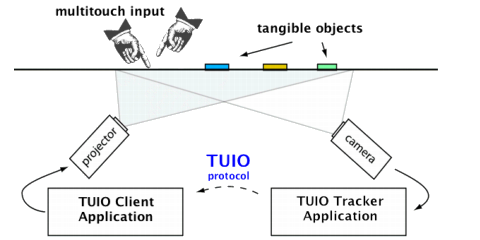
\includegraphics[width=.8\textwidth]{images/mt-diagram.png}
  \caption{This is a multitouch table!}\label{fig:mtdiagram}
\end{figure}
\subsection{Software}
The multitouch table uses The Beta, from the NUI Group \cite{NUI}, to process the video stream from the webcam. The Beta, tbeta for short, is an open source tool that analyzes a video to find tracking data for objects it recognizes as fingers or cursor devices. The software provides a great deal of control over the video parameters (high-pass filter, amplification, threshold, etc.) that adapts well to many types of multitouch displays.

Tbeta outputs the tracking data using the TUIO protocol \cite{TUIO}, which is an open framework for receiving input events in various programming environments. For this project, the TUIO events sent by tbeta were received using the open source Java TUIO library in a Processing sketch. 
